\documentclass[10pt,a4paper]{article}
\usepackage[utf8]{inputenc}
\usepackage[italian]{babel}
\usepackage{amsmath}
\usepackage{amsfonts}
\usepackage{amssymb}
%aggiungi pacchetto che commenti
\usepackage{comment}
\usepackage{graphicx}
\usepackage[left=2cm,right=2cm,top=2cm,bottom=2cm]{geometry}
\newcommand{\rem}[1]{[\emph{#1}]}
\newcommand{\exn}{\phantom{xxx}}

\author{Gruppo 23 \\ Alessandro Costanzo Ciano, Luca Palumbo}
\title{Relazione di laboratorio: esercitazione D3}
\begin{document}
\date{30 aprile 2024}
\maketitle

\section{Scopo dell'esperienza}
L'obbiettivo dell'esperienza è la realizzazione di un circuito che gestisca un semaforo come applicazione del concetto di una macchina a stati finiti (FSM) di Mealy. Il semaforo deve avere due modalità di funzionamento: "ABILITATO" o "DISABILITATO": nella modalità ABILITATO la sequenza degli stati, ripetuta ciclicamente, deve essere: LED verde acceso, LED verde e giallo accesi, LED rosso acceso. Nella modalità DISABILITATO la sequenza deve essere: LED giallo spento, LED giallo acceso. Tutti gli stati devono durare 1 impulso di clock. La modalità di funzionamento viene determinata tramite un interruttore che genera il segnale di abilitazione ("E"=enable). Si è scelto di utilizzare un segnale E attivo alto.

\section{Progettazione e realizzazione del circuito}
Si è disegnato il diagramma a stati del circuito e le relative transizioni, scegliendo di utilizzare 2 bit per la codifica degli stati (fig. \ref{fig1}). Si è scritta la tabella di verità delle transizioni di stato e delle uscite in relazione allo stato dei FF e degli ingressi (E), come riportato in fig. \ref{fig2}. Utilizzando le mappe di Karnaugh si sono definite le funzioni logiche che rappresentano le transizioni e le uscite (fig. \ref{fig3}, \ref{fig4}, \ref{fig5}). Si è costruito il circuito utilizzando gli integrati disponibili, un DIP-switch per il segnale di abilitazione e i LED. Si è generato il clock con un DIO dell'AD2 e si sono inviati al logic analyzer dell'AD2 sia il segnale di abilitazione sia le tre uscite V-G-R.


\begin{figure}[htp]
    \begin{center}
    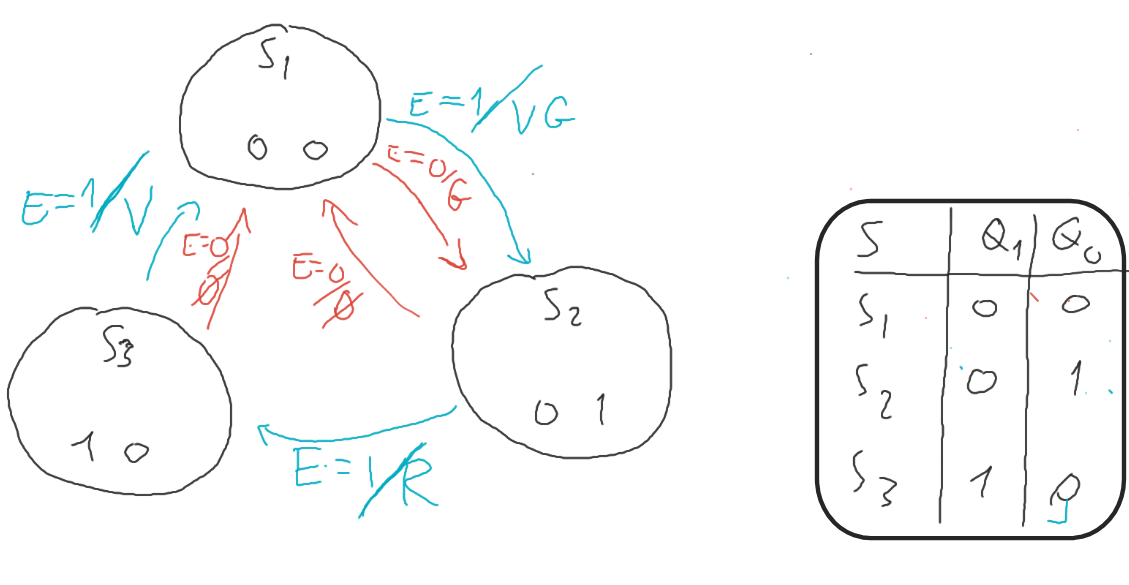
\includegraphics[scale=0.25]{fig1.png}
    \caption{Diagramma a stati del circuito.}
    \label{fig1}
    \end{center}
\end{figure}

\begin{figure}[htp]
    \begin{center}
    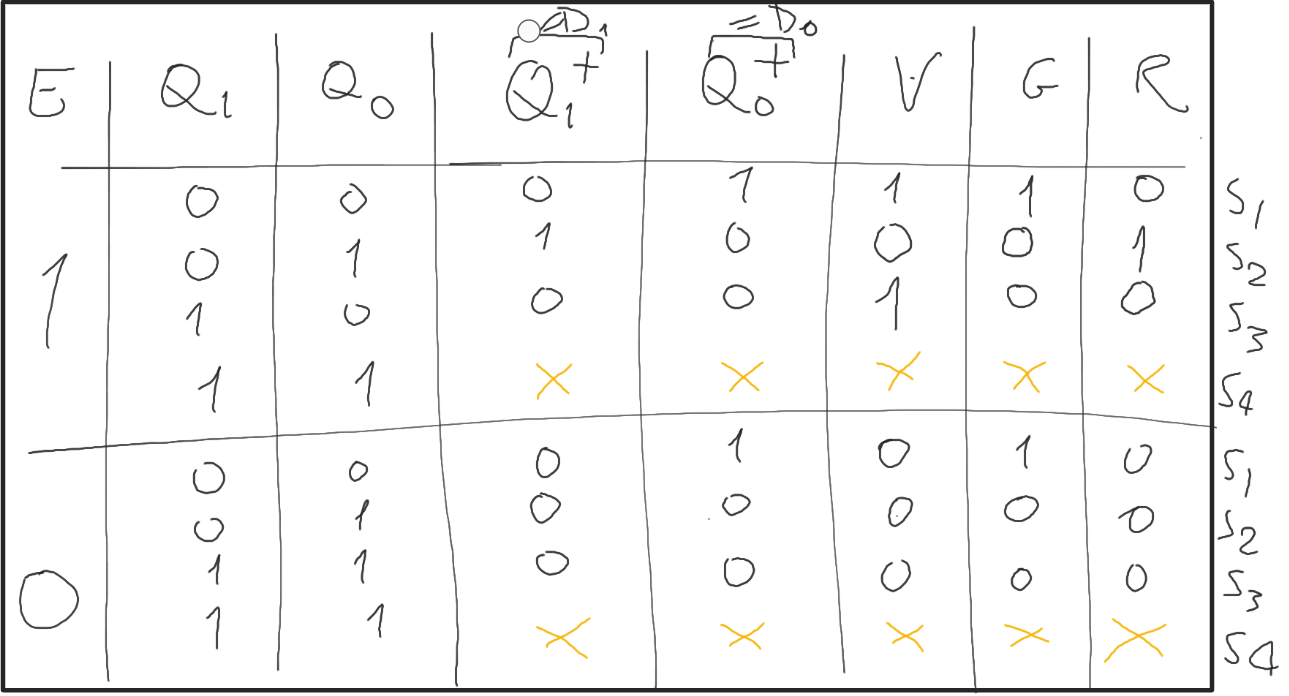
\includegraphics[scale=0.25]{fig2.png}
    \caption{Tabella di verità delle transizioni di stato e delle uscite.}
    \label{fig2}
    \end{center}
\end{figure}

\begin{figure}[htp]
    \begin{center}
    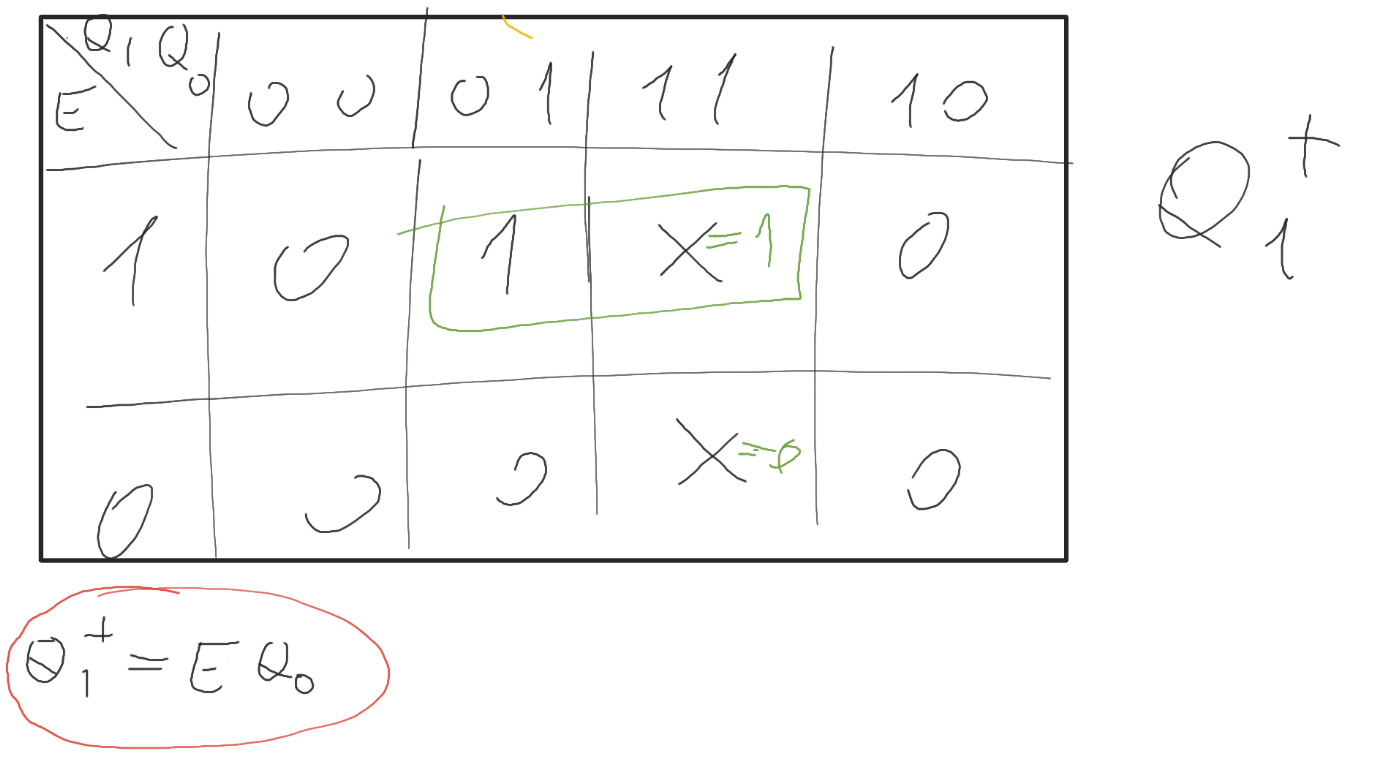
\includegraphics[scale=0.25]{fig3.png}
    \caption{Mappe di Karnaugh per la funzione logica del prossimo stato $Q_1^+$.}
    \label{fig3}
    \end{center}
\end{figure}

\begin{figure}
    \begin{center}
    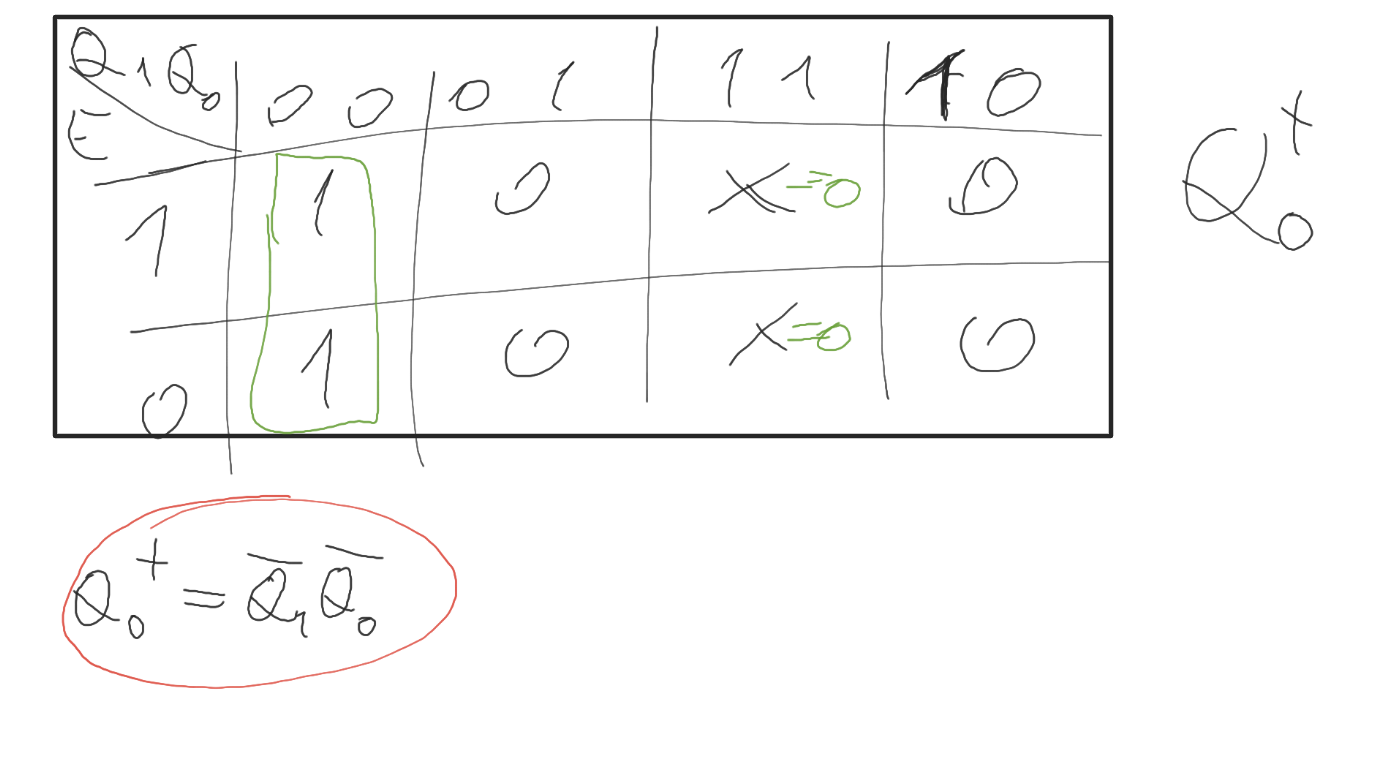
\includegraphics[scale=0.25]{fig4.png}
    \caption{Mappe di Karnaugh per la funzione logica del prossimo stato $Q_0^+$.}
    \label{fig4}
    \end{center}
\end{figure}

\begin{figure}
    \begin{center}
    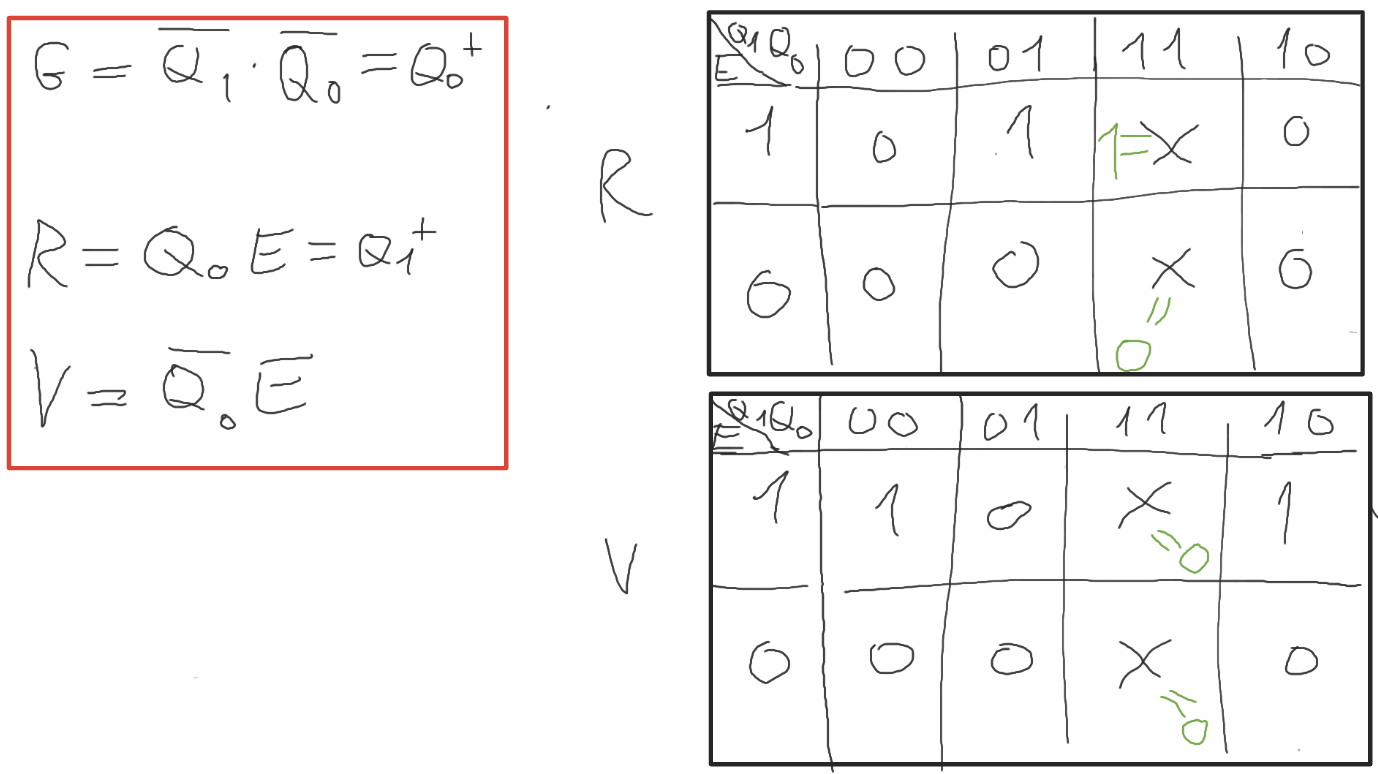
\includegraphics[scale=0.25]{fig5.png}
    \caption{Mappe di Karnaugh per le funzioni logiche del led rosso e verde (per il led giallo era determinabile ad occhio ponendo i “don’t care” a 0).}
    \label{fig5}
    \end{center}
\end{figure}

\section{Verifica del funzionamento}
In figura 6 si riporta lo schema circuitale, si noti che è stata inserita una resistenza da 1 $k\Omega$ dopo lo switch per fissare l'enable come segnale basso nel caso dello switch aperto. Per il led giallo è stata utlizzata una resistenza dedicata: questo per massimizzare la luminosità dei led giallo e verde quando sono accesi contemporaneamente.

\begin{figure}
    \begin{center}
    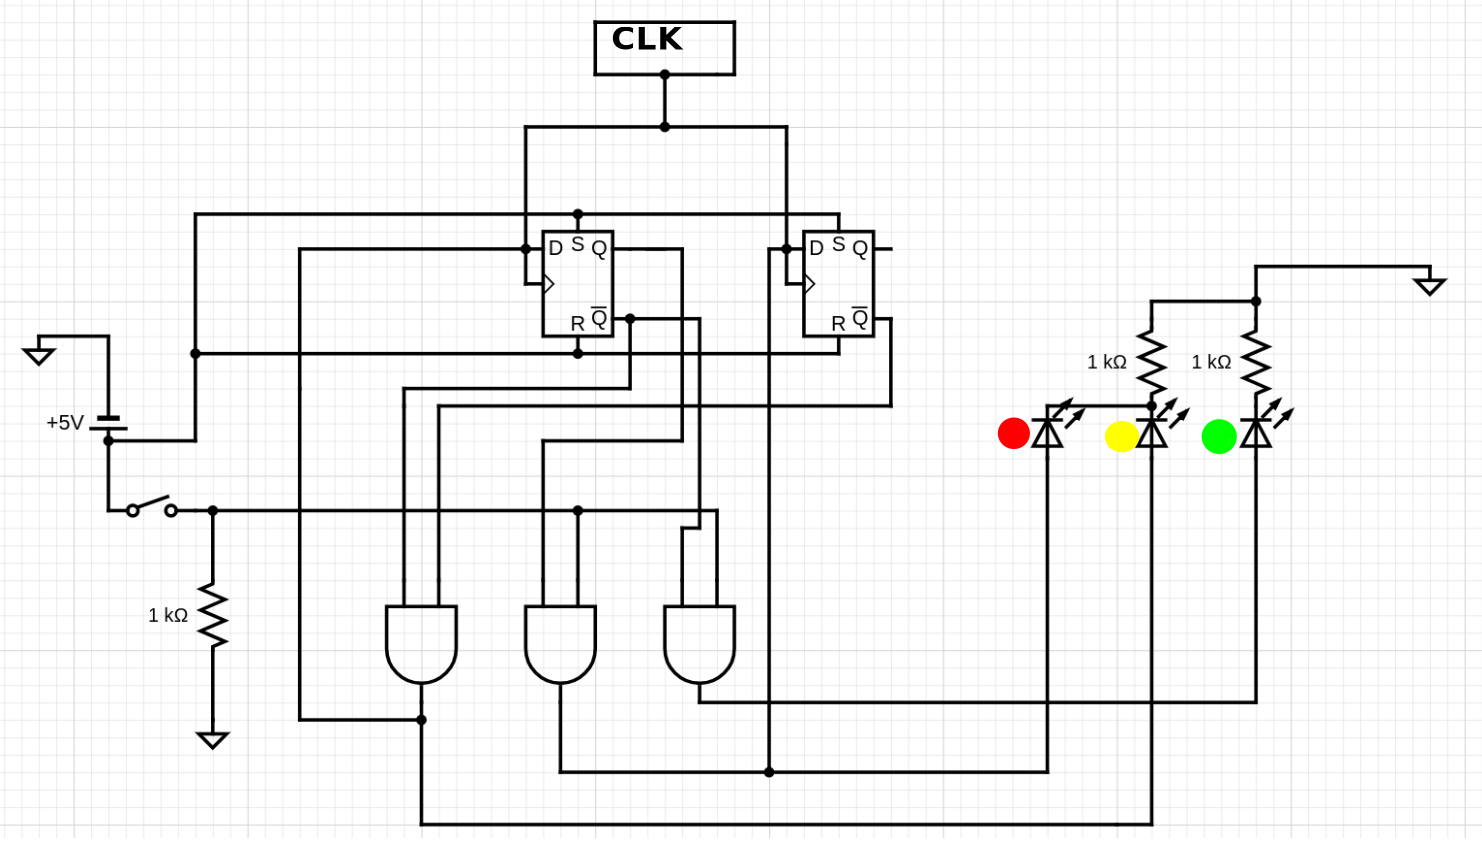
\includegraphics[scale=0.25]{fig6.png}
    \caption{Schema circuitale.}
    \label{fig6}
    \end{center}
\end{figure}

\begin{figure}
    \begin{center}
    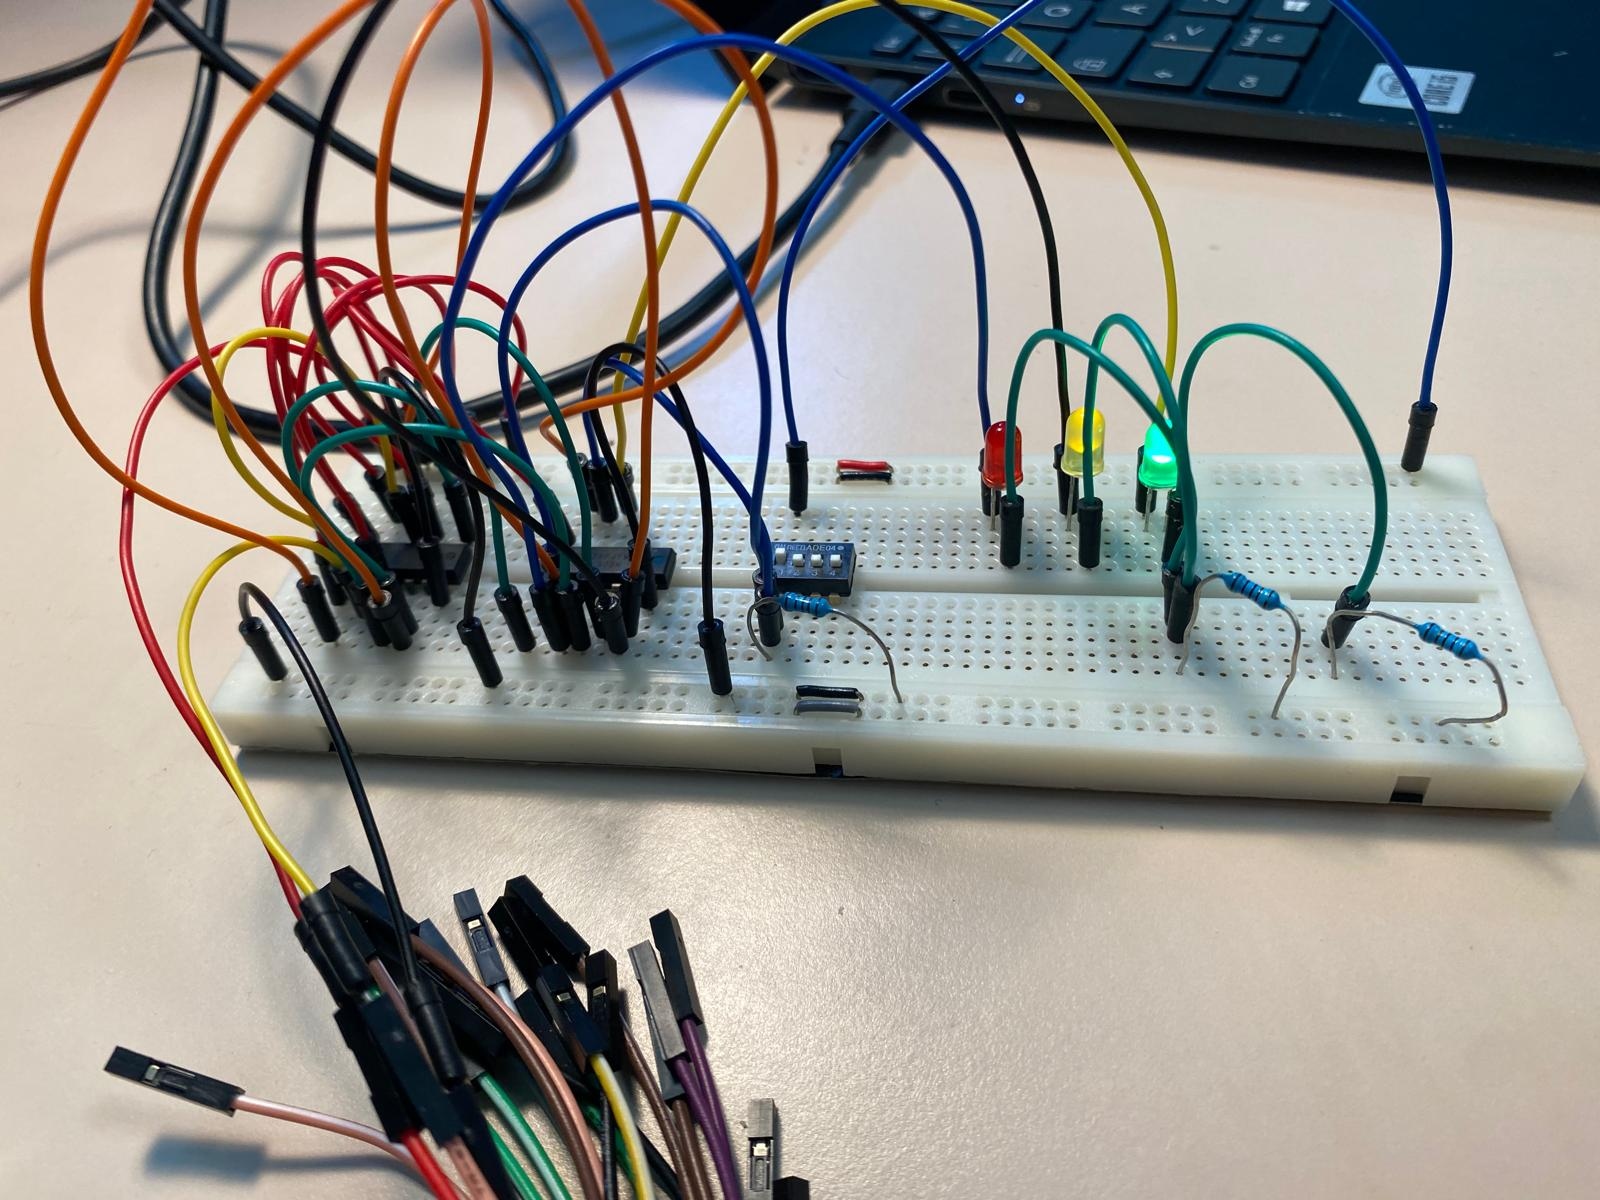
\includegraphics[scale=0.20]{WhatsApp Image 2024-04-30 at 15.05.28 (1).jpeg}
    \caption{Circuito reale 1.}
    \label{fig6}
    \end{center}
\end{figure}

\begin{figure}
    \begin{center}
    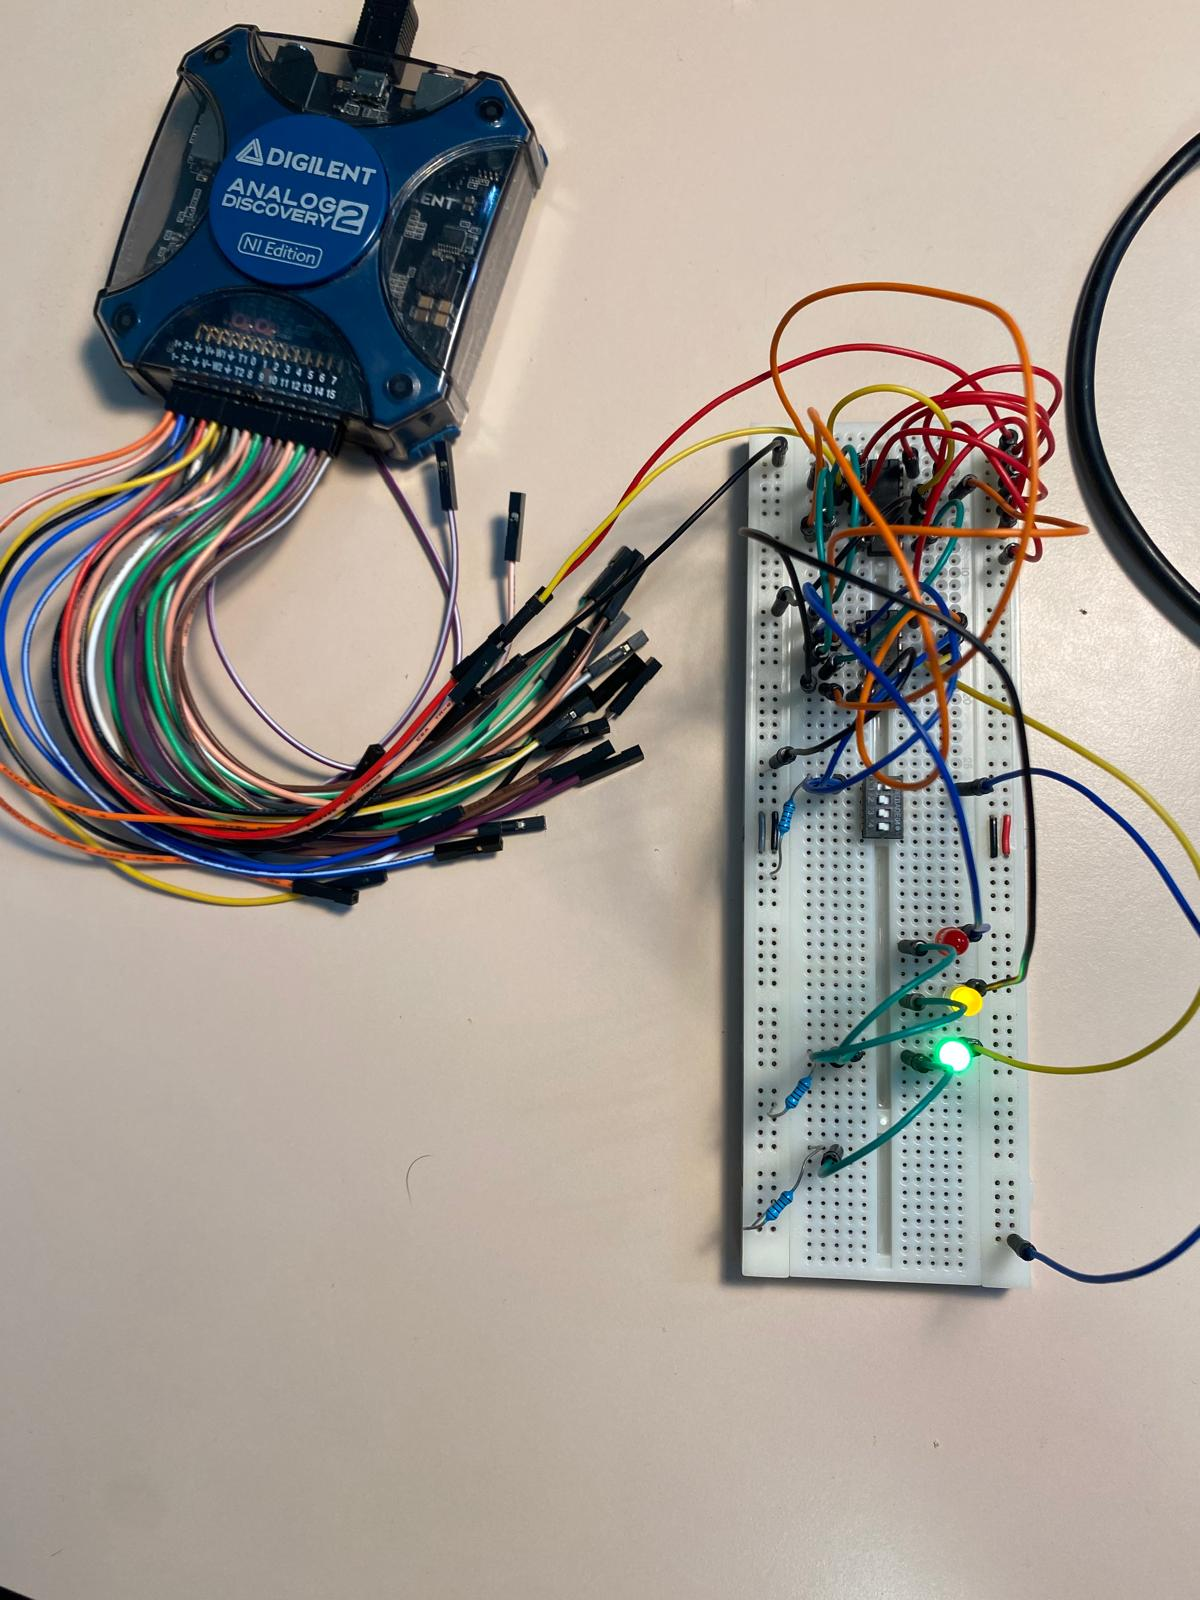
\includegraphics[scale=0.20]{WhatsApp Image 2024-04-30 at 15.05.28.jpeg}
    \caption{Circuito reale 2.}
    \label{fig6}
    \end{center}
\end{figure}

\begin{figure}
    \begin{center}
    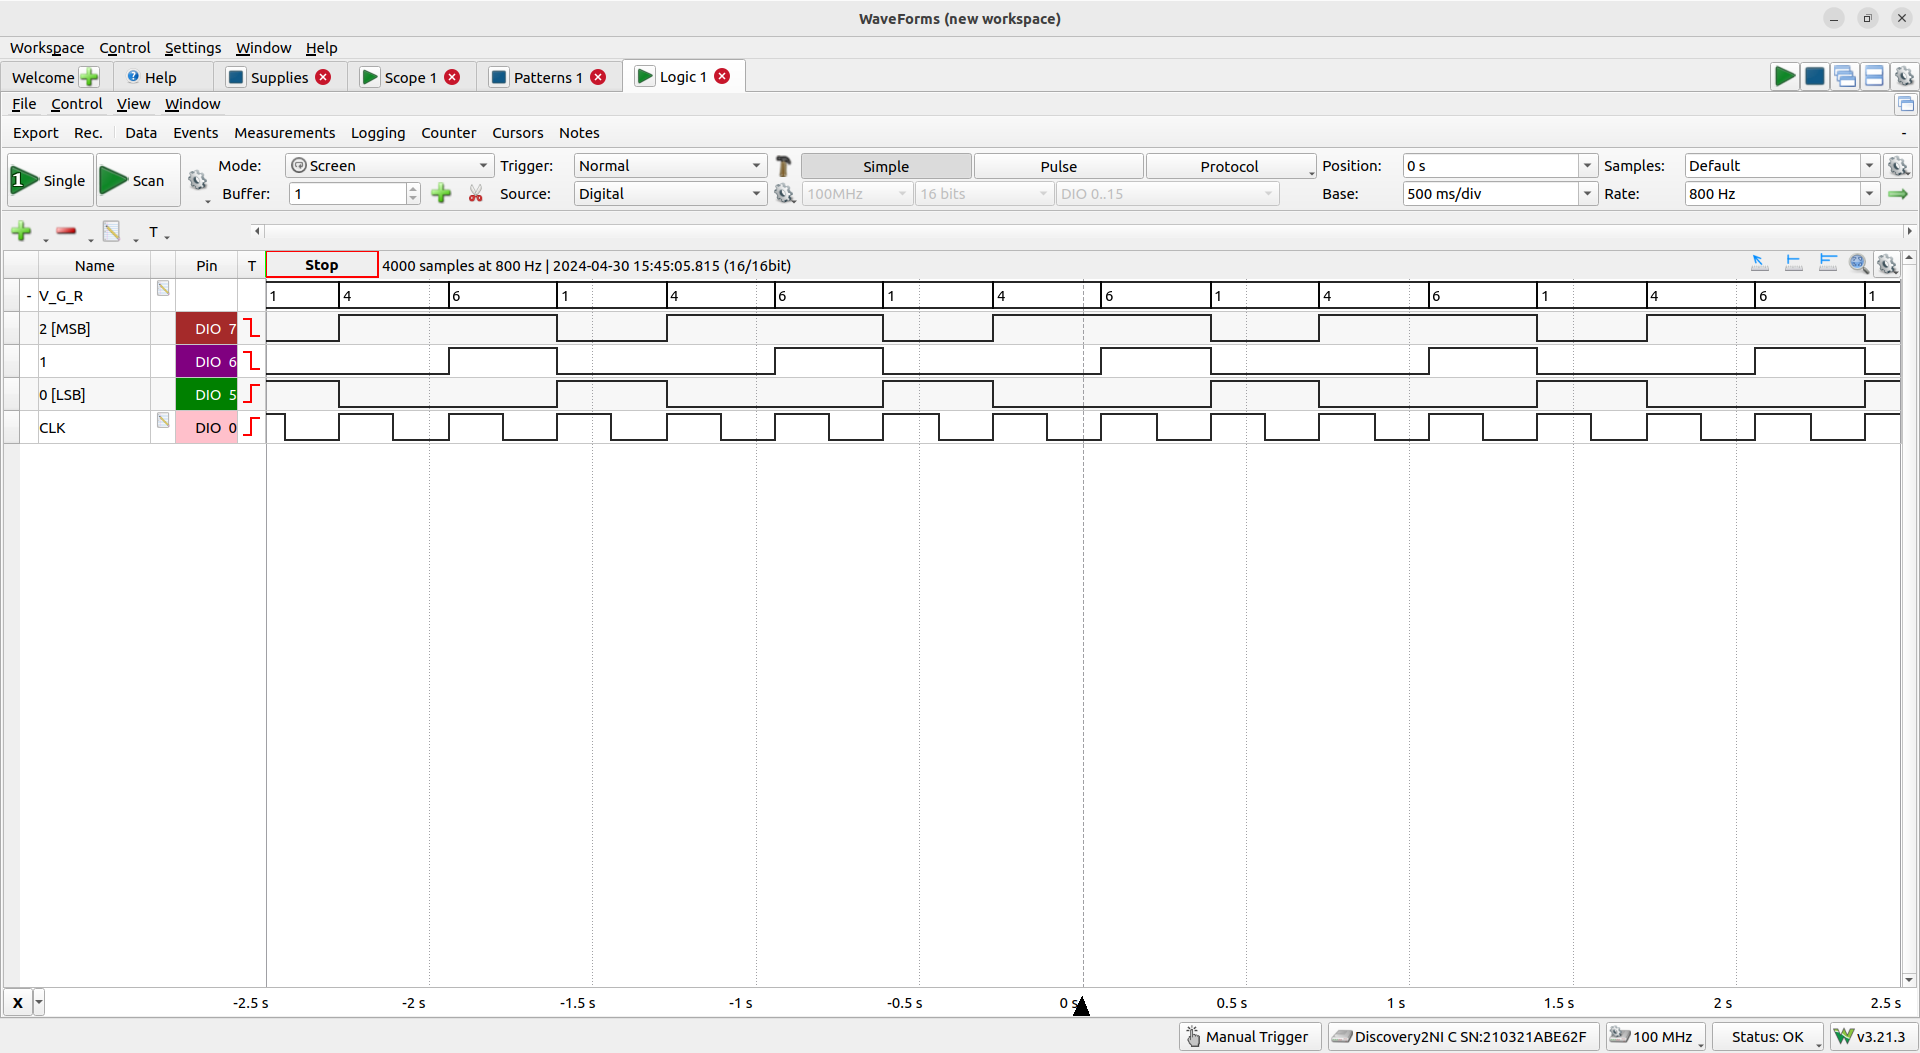
\includegraphics[scale=0.20]{fig7.png}
    \caption{Static IO del circuito per enable E = 1. Sono riportati i segnali di Clock e i tre segnali di uscita V (DIO 7), G (DIO 6), R (DIO 5).}
    \label{fig6}
    \end{center}
\end{figure}

\begin{figure}
    \begin{center}
    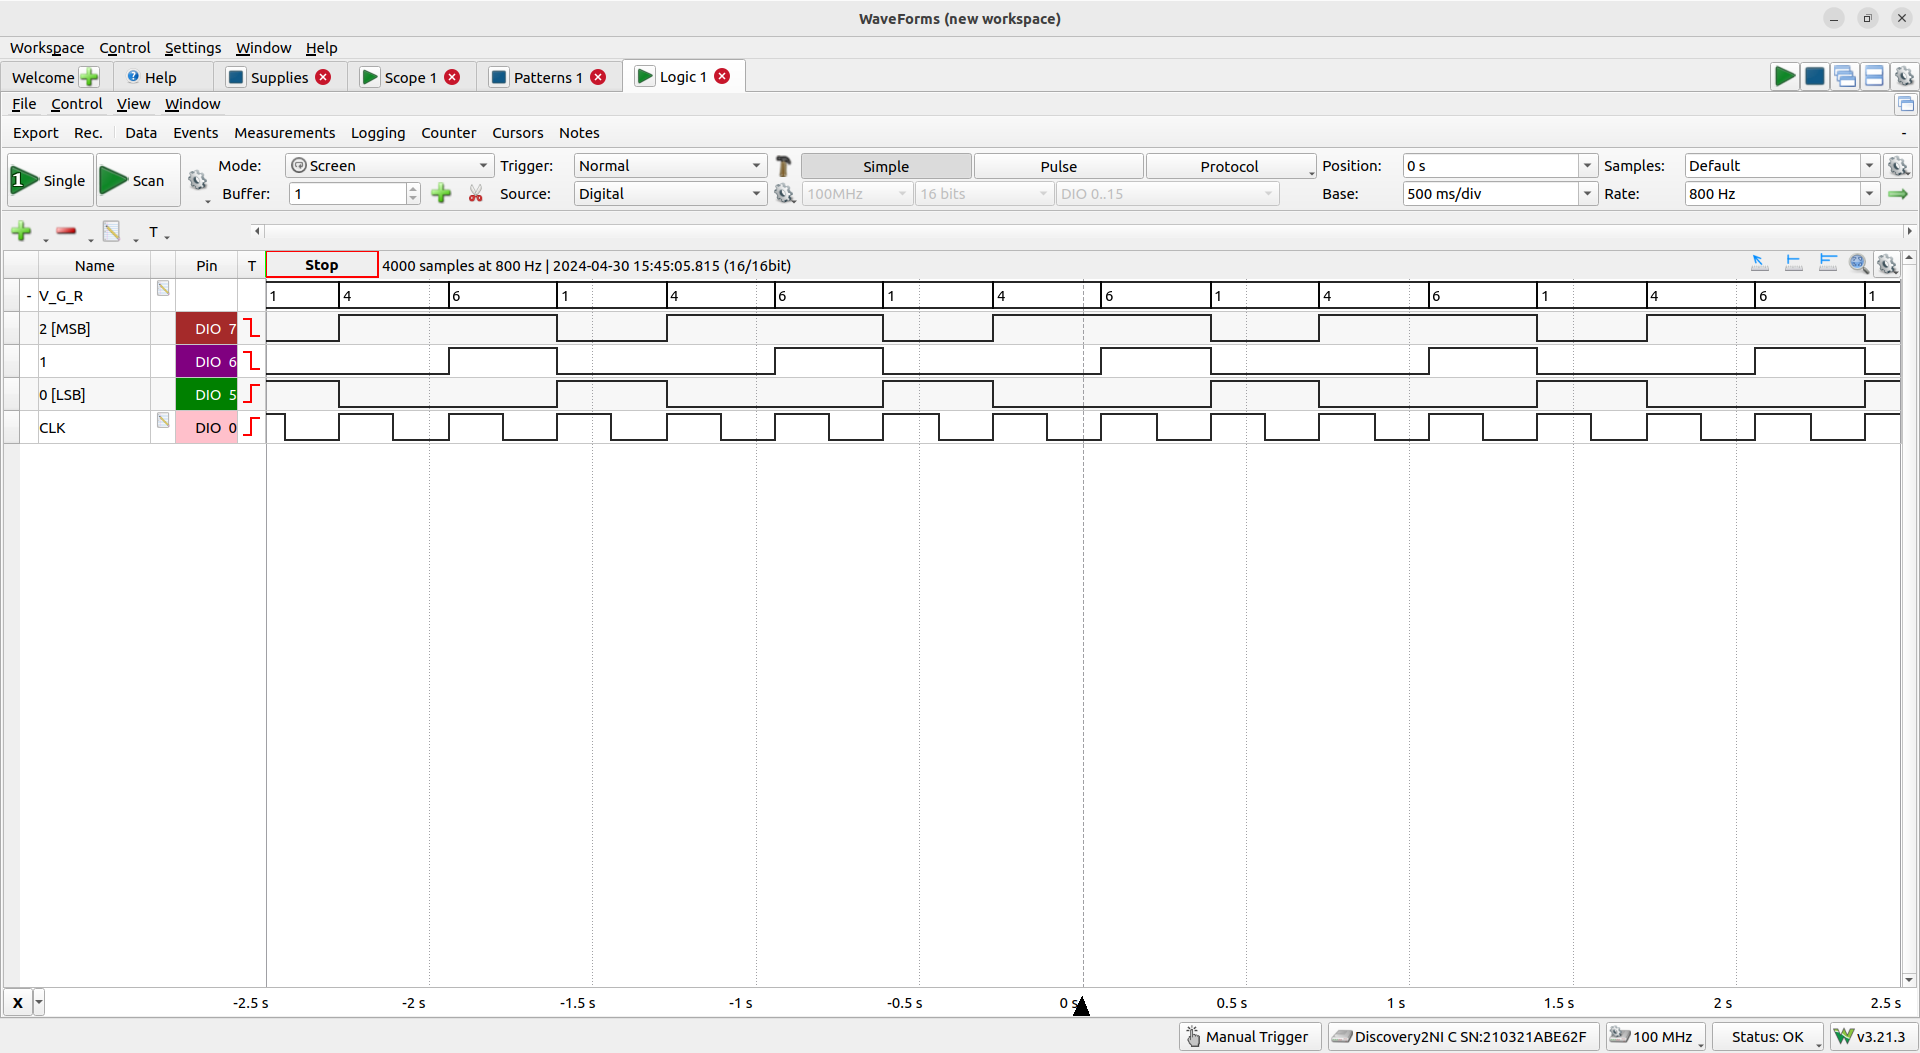
\includegraphics[scale=0.20]{fig7.png}
    \caption{Static IO del circuito per enable E = 0.}
    \label{fig6}
    \end{center}
\end{figure}


%da qui le indicazioni da seguire
\begin{comment}
Laboratorio di Fisica 3 
Prof. D.Nicolo`, Prof. C.Roda
Esercitazione N. D3
Macchina a Stati Finiti: semaforo
Questa esercitazione prevede la progettazione ed implementazione di un circuito che gestisce un 
semaforo come applicazione del concetto di una macchina a stati finiti (FSM). Dopo aver costruito 
il circuito con i componenti fisici, si dovrà implementare la FSM attraverso la l'utilizzo della ROM 
all'interno dell'Analog Discovery 2.
Alcune avvertenze:
A. Si raccomanda di eseguire un montaggio ordinato e pianificare lo spazio sulla basetta.
B. Si raccomanda di collegare gli ingressi asincroni (preset e clear) dei FF alla tensione di 
alimentazione VCC, per evitare di avere reset o clear spuri.
C. L’esercitazione prevede la costruzione autonoma di tabelle di verità e di circuiti elettrici: siate 
ordinati e sistematici, e indicate chiaramente nella relazione che cosa avete realizzato. Riportate 
sullo schema elettrico i numeri dei pin relativi agli integrati, accertandovi di aver fatto tutti i 
collegamenti comprese le alimentazioni (GND e VCC).
Materiale a disposizione - Consultare i data-sheet per le piedinature degli integrati.
• 2 Integrati 74LS74 – 2 FF di tipo D, 1 Integrato 74LS00 – 4 Porte NAND
• 1 Integrato 74LS08 – 4 Porte AND, 1 Integrato 74LS32 – 4 Porte OR
• 3 LED: verde, rosso, giallo; 1 switch 4 bit
Specifiche di funzionamento del semaforo 
Il semaforo deve avere due modalità di funzionamento: “ABILITATO” o “DISABILITATO”. 
Nella modalità ABILITATO la sequenza degli stati, ripetuta ciclicamente, deve essere:
• LED verde acceso, LED verde e giallo accesi, LED rosso acceso
Nella modalità DISABILITATO la sequenza deve essere:
• LED giallo spento, LED giallo acceso
Tutti gli stati devono durare 1 impulso di clock. 
La modalità di funzionamento viene determinata tramite un interruttore che genera il segnale di 
abilitazione (“E”=enable). Si può scegliere se il segnale E sia attivo alto oppure attivo basso, ma 
fare attenzione ad essere consistenti nella definizione e nella analisi.
Si richiede di implementare il semaforo come una Macchina a stati finiti di Mealy (si noti 
che è possibile trovare una soluzione a tre stati).
Procedimento per l’implementazione del semaforo con circuiti integrati: 
a) Disegnare il diagramma a stati del circuito e le relative transizioni. Partite disegnando le 
transizioni per lo stato abilitato e poi completate il diagramma con le transizioni per lo stato 
disabilitato. Riportate il diagramma nella relazione 
b) Associate ai vari stati (S) la codifica in termini di bit, che saranno implementati nel registro 
costituito dai FF D (potete utilizzare fino a 4 bit) e definite se il segnale di Enable (E) è 
attivo alto o basso. Riportate nella relazione la vostra scelta e completate il diagramma di 
stato con le codifiche da voi scelte. Si noti che la scelta della codifica degli stati influisce 
sulla complessità della logica combinatoria di output.
c) Scrivete la tabella di verità delle transizioni di stato e delle uscite in relazione allo stato dei 
FF e degli ingressi (E).
d) Se necessario potete utilizzate le mappe di Karnaugh per aiutarvi a minimizzare la logica 
combinatoria nel definire le funzioni logiche che rappresentano le transizioni: Sn+1 = f(Sn, 
ingressi) e le funzioni logiche che rappresentano le uscite Outi = f(Sn, ingressi). Riportate 
tutta la vostra analisi nella relazione.
e) Specificate come avete utilizzato gli stati “don’t care” e spiegate le vostre scelte.
f) Costruite il circuito, utilizzando i circuiti integrati disponibili, un DIP-switch (vero non in 
SW) per il segnale di abilitazione ed i LED (veri). Generate il clock con un DIO dell'AD2 ed 
inviate al logic analyzer dell'AD2 sia il segnale di abilitazione sia le tre uscite V-G-R. 
Eseguite un filmato del circuito con un clock lento, da caricare sulla chat del gruppo per 
dimostrare il funzionamento.
g) Osservate le uscite V-G-R a dei canali DIO dell'AD2 in static IO e verificate il 
funzionamento. Osservate i segnali nel logic analyzer e allegate alla relazione gli screenshot 
necessari alla dimostrazione del funzionamento del vostro circuito.
\end{comment}
\end{document}

